\documentclass[xcolor=table, 10pt, aspectratio=169]{beamer}

%\usepackage{arev}
\usepackage{amsmath,amssymb,amscd}
\usepackage{dsfont}
\usepackage{mathrsfs}
\usepackage{yfonts}
\usepackage{bm}
\usepackage{graphicx}
\usepackage{tabularx}
\usepackage{animate}

%\usepackage{xeCJK}
%\usepackage{fontspec}
%\newfontfamily\cjkfont{PingFang SC}
%\setCJKmainfont{PingFang SC}
\newcolumntype{x}{>{\centering\arraybackslash}X}
\renewcommand{\arraystretch}{1.5}

\usepackage{tikz}
	\usetikzlibrary{calc}
	\usetikzlibrary{arrows,shapes, positioning, matrix}
	\usetikzlibrary{decorations.markings}
	\tikzstyle arrowstyle=[scale=1]
	\tikzstyle directed=[postaction={decorate,decoration={markings,
 	   mark=at position .15 with {\arrow[arrowstyle]{stealth}}}}]
\tikzstyle string=[thick,postaction={decorate,decoration={markings,
    mark=at position .55 with {\arrow[arrowstyle]{stealth}}}}]
\tikzstyle dual_string=[dashed,postaction={decorate,decoration={markings,
    mark=at position .55 with {\arrow[arrowstyle]{stealth}}}}]

\tikzstyle dw=[thick,postaction={decorate,decoration={markings,
    mark=at position 1 with {\arrow[arrowstyle]{stealth}}}}]
\tikzstyle group=[mbg]

\usepackage{pgffor}
\newcommand{\mb}[1]{\mathbf{#1}}
\renewcommand{\cal}[1]{\mathcal{#1}}

\newcommand{\ag}[2]{#1_\mb{#2}}
\newcommand{\cohosub}[1]{\scalebox{0.72}{\textswab{#1}}}
\newcommand{\cohosubsub}[1]{\scalebox{0.6}{\textswab{#1}}}
\newcommand{\coho}[1]{\textswab{#1}}


\mode<presentation>
{
  %\usetheme{Warsaw}
  % or ...
  %\useoutertheme{rectangle}
  \setbeamertemplate{frametitle}[default][center]
  \defbeamertemplate{itemize item}{flat}{\begin{pgfpicture}{-1ex}{0ex}{1ex}{2ex}
      \pgfpathcircle{\pgfpoint{0pt}{.6ex}}{0.6ex}
      \pgfusepath{fill}
    \end{pgfpicture}%
  }
  \defbeamertemplate{itemize subitem}{flat}{\footnotesize\raise0.5pt\hbox{\textbullet}}
  \defbeamertemplate{itemize subsubitem}{flat}{\footnotesize\raise0.5pt\hbox{\textbullet}}

  %\useinnertheme{circles}
  \setbeamertemplate{items}[flat]
  \setbeamertemplate{sections/subsections in toc}[circle]
  \setbeamertemplate{blocks}[rounded]
  \setbeamertemplate{title page}[default][colsep=-4bp,rounded=true]
  \setbeamertemplate{part page}[default][colsep=-4bp,rounded=true]
  \setbeamercovered{transparent}
  %\usecolortheme{spruce}
  %\definecolor{THU}{RGB}{116,61,130}
  \definecolor{mbg}{RGB}{0,0,160}
  \setbeamercolor*{palette primary}{fg=white,bg=mbg}
  \setbeamercolor*{titlelike}{parent=palette primary}
  \setbeamercolor*{structure}{fg=mbg}
  \setbeamercolor{frametitle}{fg=white,bg=mbg}
  % or whatever (possibly just delete it)
  \setbeamercolor{block title}{bg=mbg,fg=white}
  \setbeamercolor{block body}{bg=mbg!15}


  \addtobeamertemplate{navigation symbols}{}{ \hspace{1em}%
    \usebeamerfont{footline}%
    \insertframenumber / \inserttotalframenumber }
}


%\usepackage[english]{babel}
% or whatever

%\usepackage[latin1]{inputenc}
% or whatever

%\usepackage{times}
%\usepackage[T1]{fontenc}
% Or whatever. Note that the encoding and the font should match. If T1
% does not look nice, try deleting the line with the fontenc.

\title[Mirror SET] % (optional, use only with long paper titles)
{Quantum spin liquids: topological order and fractionalized excitations}

\author[Y Qi] % (optional, use only with lots of authors)
{Yang~Qi}
% - Give the names in the same order as the appear in the paper.
% - Use the \inst{?} command only if the authors have different
%   affiliation.

\institute[MIT] % (optional, but mostly needed)
{
  Massachusetts Institute of Technology\\
  Joining Fudan University in 2017
}
% - Use the \inst command only if there are several affiliations.
% - Keep it simple, no one is interested in your street address.

%\date{2016 Annual Meeting of Fudan CFTPP} % (optional, should be abbreviation of conference name)
%{Fudan University, Oct 13 2015}
\date{Shanghai Tech University, July 24, 2017.}
% - Either use conference name or its abbreviation.
% - Not really informative to the audience, more for people (including
%   yourself) who are reading the slides online

\subject{Theoretical Physics}
% This is only inserted into the PDF information catalog. Can be left
% out.



% If you have a file called "university-logo-filename.xxx", where xxx
% is a graphic format that can be processed by latex or pdflatex,
% resp., then you can add a logo as follows:

%\pgfdeclareimage[height=1cm]{university-logo}{fudan}
%\logo{\pgfuseimage{university-logo}}



% Delete this, if you do not want the table of contents to pop up at
% the beginning of each subsection:
\AtBeginSection[]
{
  \begin{frame}<beamer>{Outline}
			\tableofcontents[currentsection,currentsubsection]
  \end{frame}
}
%\AtBeginSubsection[]
%{
 % \begin{frame}<beamer>{Outline}
  %  \tableofcontents[currentsection,currentsubsection]
  %\end{frame}
%}


\begin{document}

\begin{frame}
  \titlepage
\end{frame}

\begin{frame}{Collaborators and References}
  Collaborators:
  \begin{itemize}
		\item Chen Fang, Institute of Physics, Chinese Academy of Science.
		\item Liang Fu, Massachusetts Institute of Technology.
    \item Meng Cheng, Yale University.
  \end{itemize}
  \begin{center}
    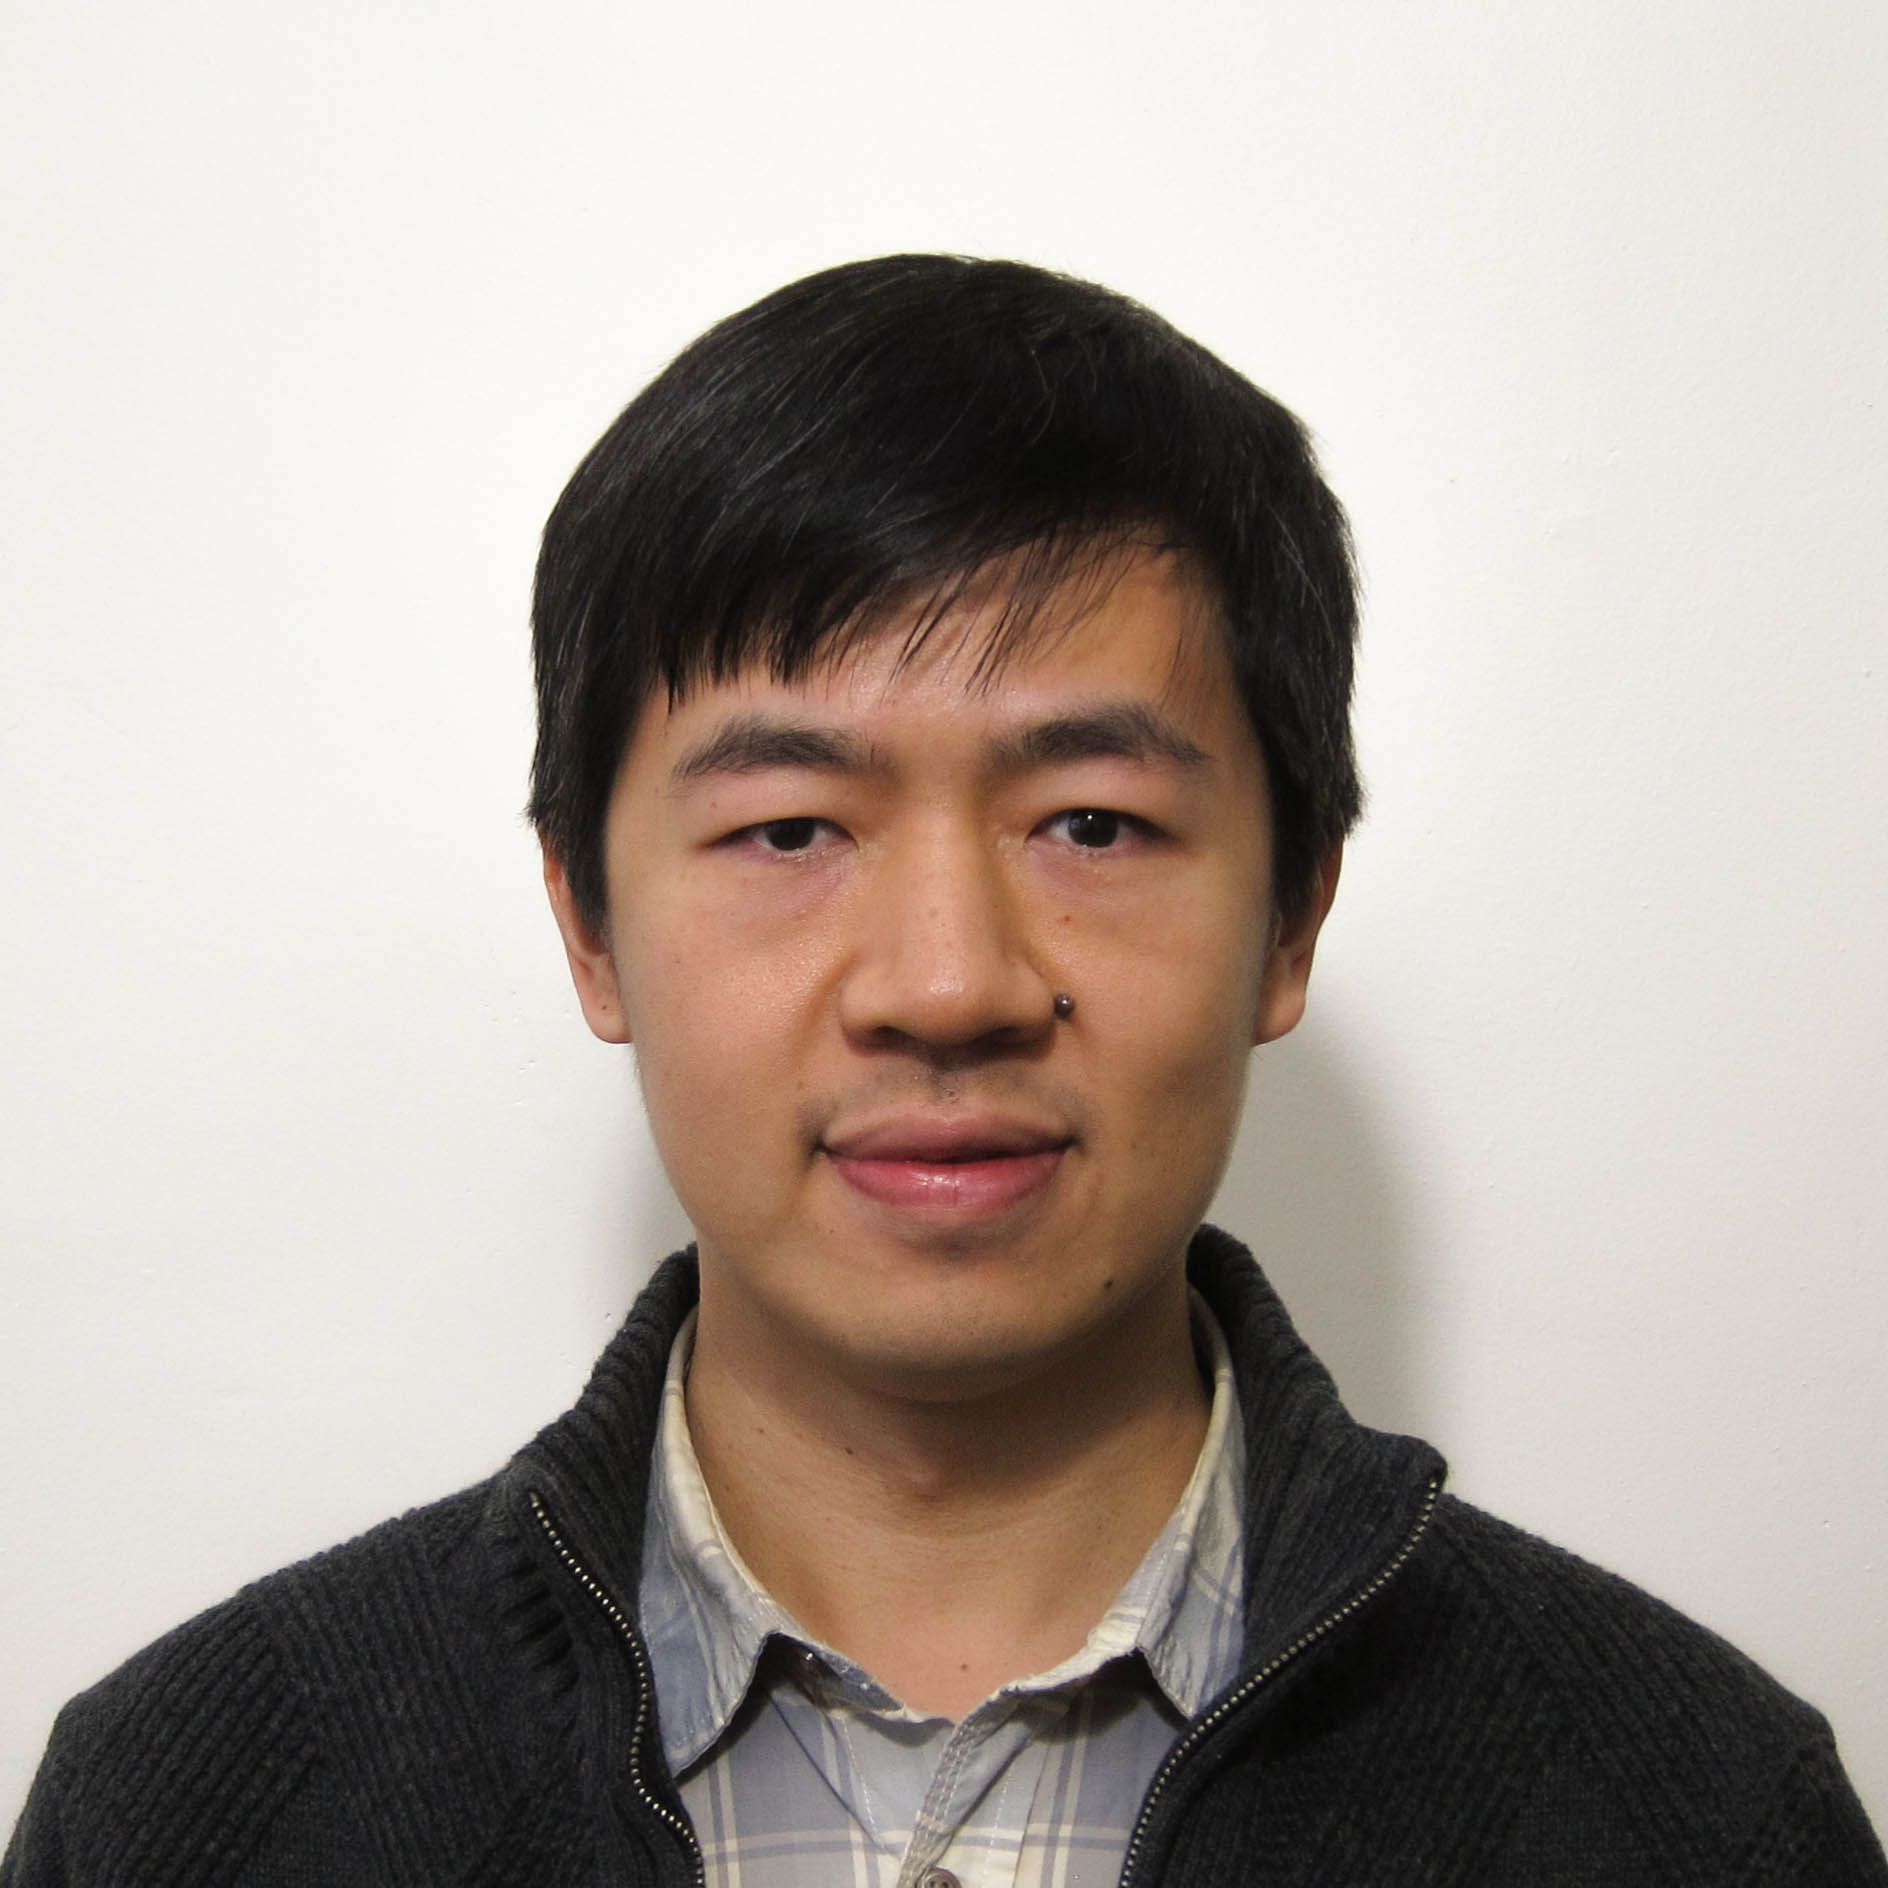
\includegraphics[height=3cm]{../people/chenfang}~~~~~
	  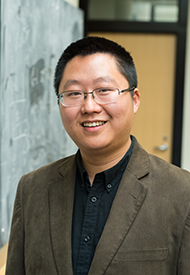
\includegraphics[height=3cm]{../people/liangfu}~~~~~
    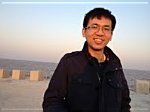
\includegraphics[height=3cm]{../people/mengcheng}
  \end{center}
  References:
  {\small
  \begin{itemize}
  \item Yang Qi, Chen Fang and Liang Fu, \href{https://arxiv.org/abs/1705.09190}{arXiv:1705.09190}.
  \item Yang Qi and Meng Cheng,
  \href{https://arxiv.org/abs/1606.04544}{arXiv:1606.04544}.
  \end{itemize}}
\end{frame}

\begin{frame}{Outline}
	%\begin{columns}
	%\column{.7\textwidth}
		\tableofcontents
  %\end{columns}
  % You might wish to add the option [pausesections]
\end{frame}

\section{Introduction: topological phases and where to find them?}

\begin{frame}{Landau's paradigm: symmetry breaking}
  Traditional phases are organized in Landau's paradigm.
  \begin{enumerate}
  \item Crystal: breaking translation symmetry.
  \item Magnet: breaking spin-rotation symmetry.
  \item Superconductor: breaking U(1) charge-conservation symmetry.
  \end{enumerate}
  \begin{center}
    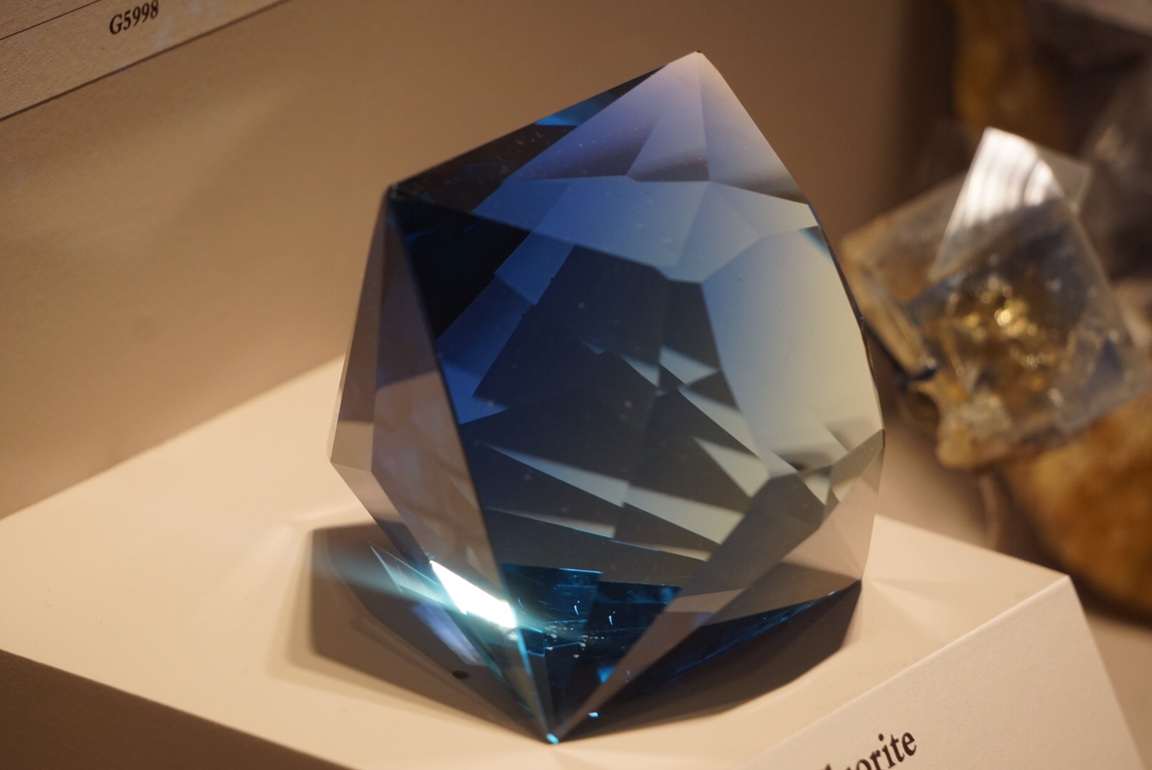
\includegraphics[height=3cm]{../resources/crystal}~~
    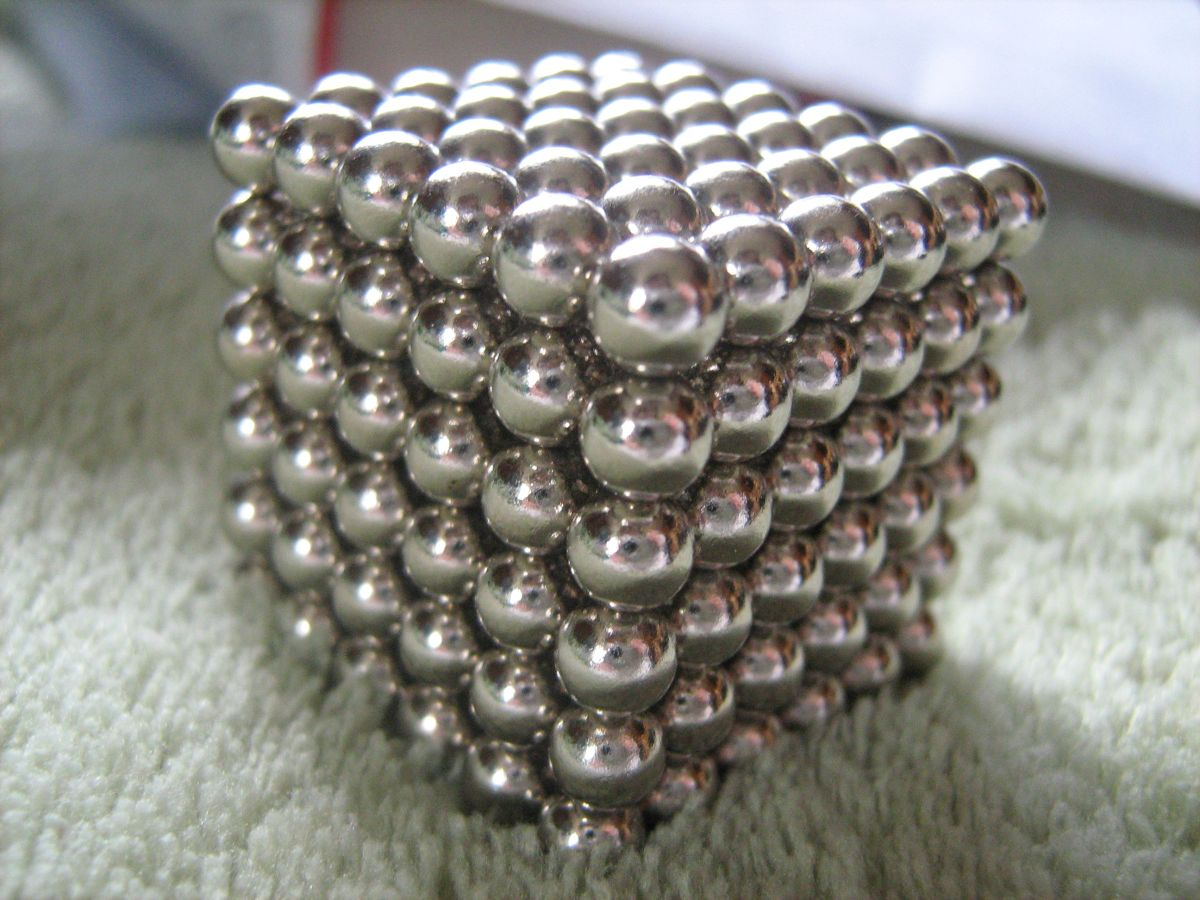
\includegraphics[height=3cm]{../resources/magnet}~~
    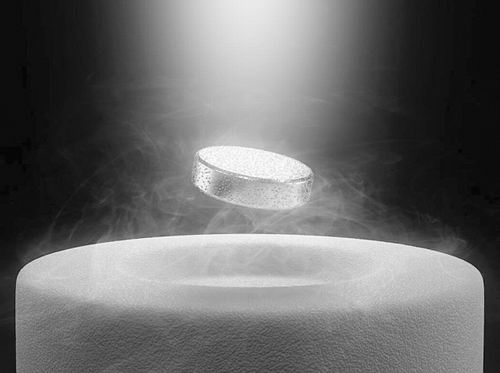
\includegraphics[height=3cm]{../resources/sc}
  \end{center}
\end{frame}

\begin{frame}
  \frametitle{Topological phases}
  Features of topological phases:
  \begin{itemize}
  \item No symmetry breaking, but still nontrivial.
  \item Long-range quantum entanglement.
  \item Anyon excitations: fractional statistics and fractional charge.
  \item Ground state degeneracy on a torus.
  \end{itemize}
  Examples of topological orders:
  \begin{enumerate}
  \item Fractional quantum hall States.
  \item Quantum spin liquids.
\end{enumerate}
\end{frame}

\begin{frame}
\frametitle{Fractional Quantum Hall}
\begin{columns}
\column{.3\textwidth}
  \begin{center}
  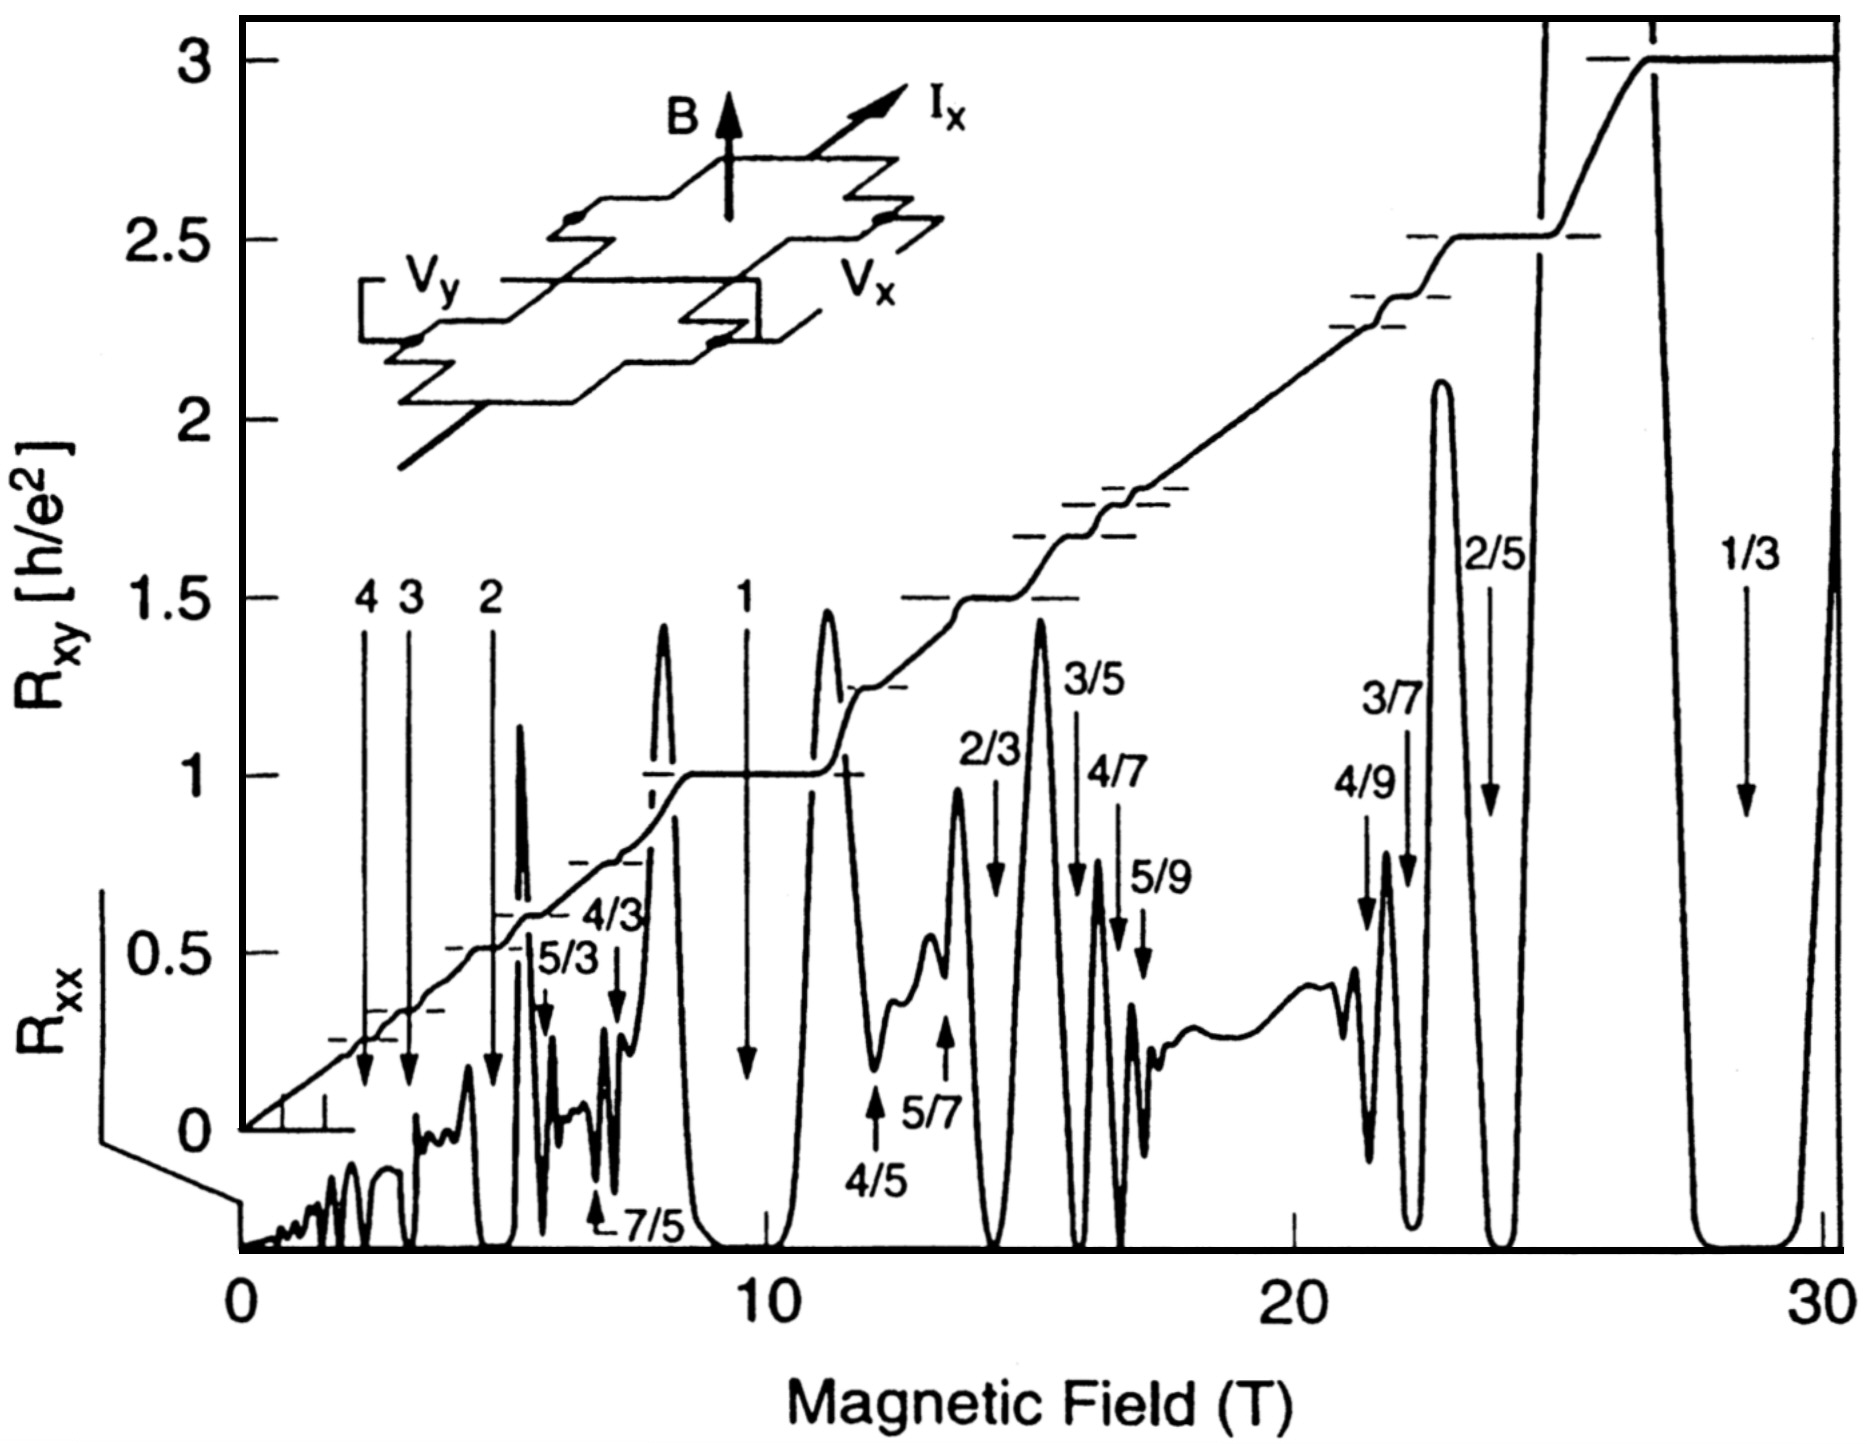
\includegraphics[width=\columnwidth]{../resources/fqhe}
  \end{center}
\column{.7\textwidth}
  \begin{itemize}
  \item Laughlin wave function:
  \[\Psi(z_1,\ldots,z_N)=\prod_{i\neq j}(z_i-z_j)^3\cdots.\]
  \item Quasiparticle excitations: charge=$\frac13$, statistics=$\frac\pi3$.
  \item Ground state degeneracy: 3-fold on a torus.
  \end{itemize}
\end{columns}
\end{frame}

\begin{frame}
\frametitle{$\mathbb Z_2$ Quantum Spin Liquid}
\begin{itemize}
\item<1-> Ground state wavefunction: superposition of all dimer configurations.
\item<3-> Long-range entanglement: use a cut encircling odd \# of sites.
\item<4-> Quasiparticle excitations: spin-$\frac12$.
\item<9-> Ground state degeneracy: 4-fold degenerate.
\end{itemize}
\begin{center}
\includegraphics<1>{../dimer/dimer_spin}
\includegraphics<2>{../dimer/dimer0}
\includegraphics<3>{../dimer/dimerloop}
\includegraphics<4>{../dimer/dimer1}
\includegraphics<5>{../dimer/dimer2}
\includegraphics<6>{../dimer/dimer3}
\includegraphics<7>{../dimer/dimer4}
\includegraphics<8>{../dimer/dimer5}
\includegraphics<9>{../dimer/dimer_cut}
\includegraphics<10>{../dimer/dimer_cut2}
\includegraphics<11>{../dimer/dimer_cut3}
\end{center}
\end{frame}

\begin{frame}
  \frametitle{Topological phases and where to find them}
  \begin{columns}
  \column{.6\textwidth}
  \begin{itemize}
    \item<1-2> Topological phases with exotic features: fractionalized quasiparticles and anyonic statistics.
    \item<1-2> Fractional quantum Hall states.
    \item<1-2> Exactly solvable models.
    \item<1> Numerical simulations of quantum spin models.
    \item<1> Materials.
  \end{itemize}
  \column{.4\textwidth}
  \begin{center}
    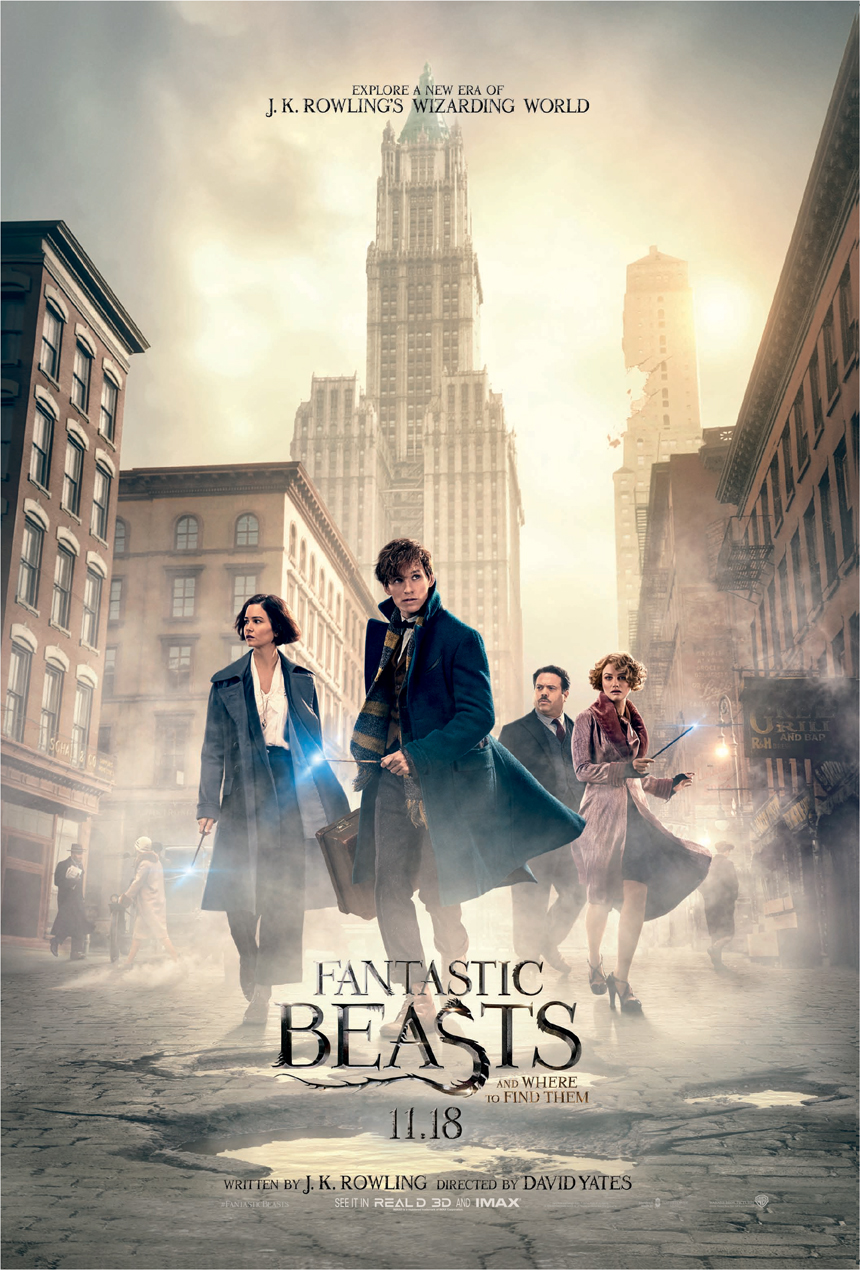
\includegraphics[width=4.5cm]{../resources/fbeasts}
  \end{center}
  \end{columns}
\end{frame}

\begin{frame}
\frametitle{Why is spin liquids so hard to find}
\begin{itemize}
\item Needs guiding principles to narrow down the search:\\
frustration, quantum spins, $\cdots$
\item Topological order is hard to detect:
\begin{itemize}
\item Entanglement: cannot detect experimentally.
\item Ground state degeneracy: cannot put the system on a torus.
\item Quasiparticles: cannot be created individually; hard to detect.
\end{itemize}
\item No-go theorems:
\begin{itemize}
\item Guarantees symmetry-protected ground state degeneracy.
\item Suggests topological order.
\end{itemize}
\end{itemize}

\begin{center}
  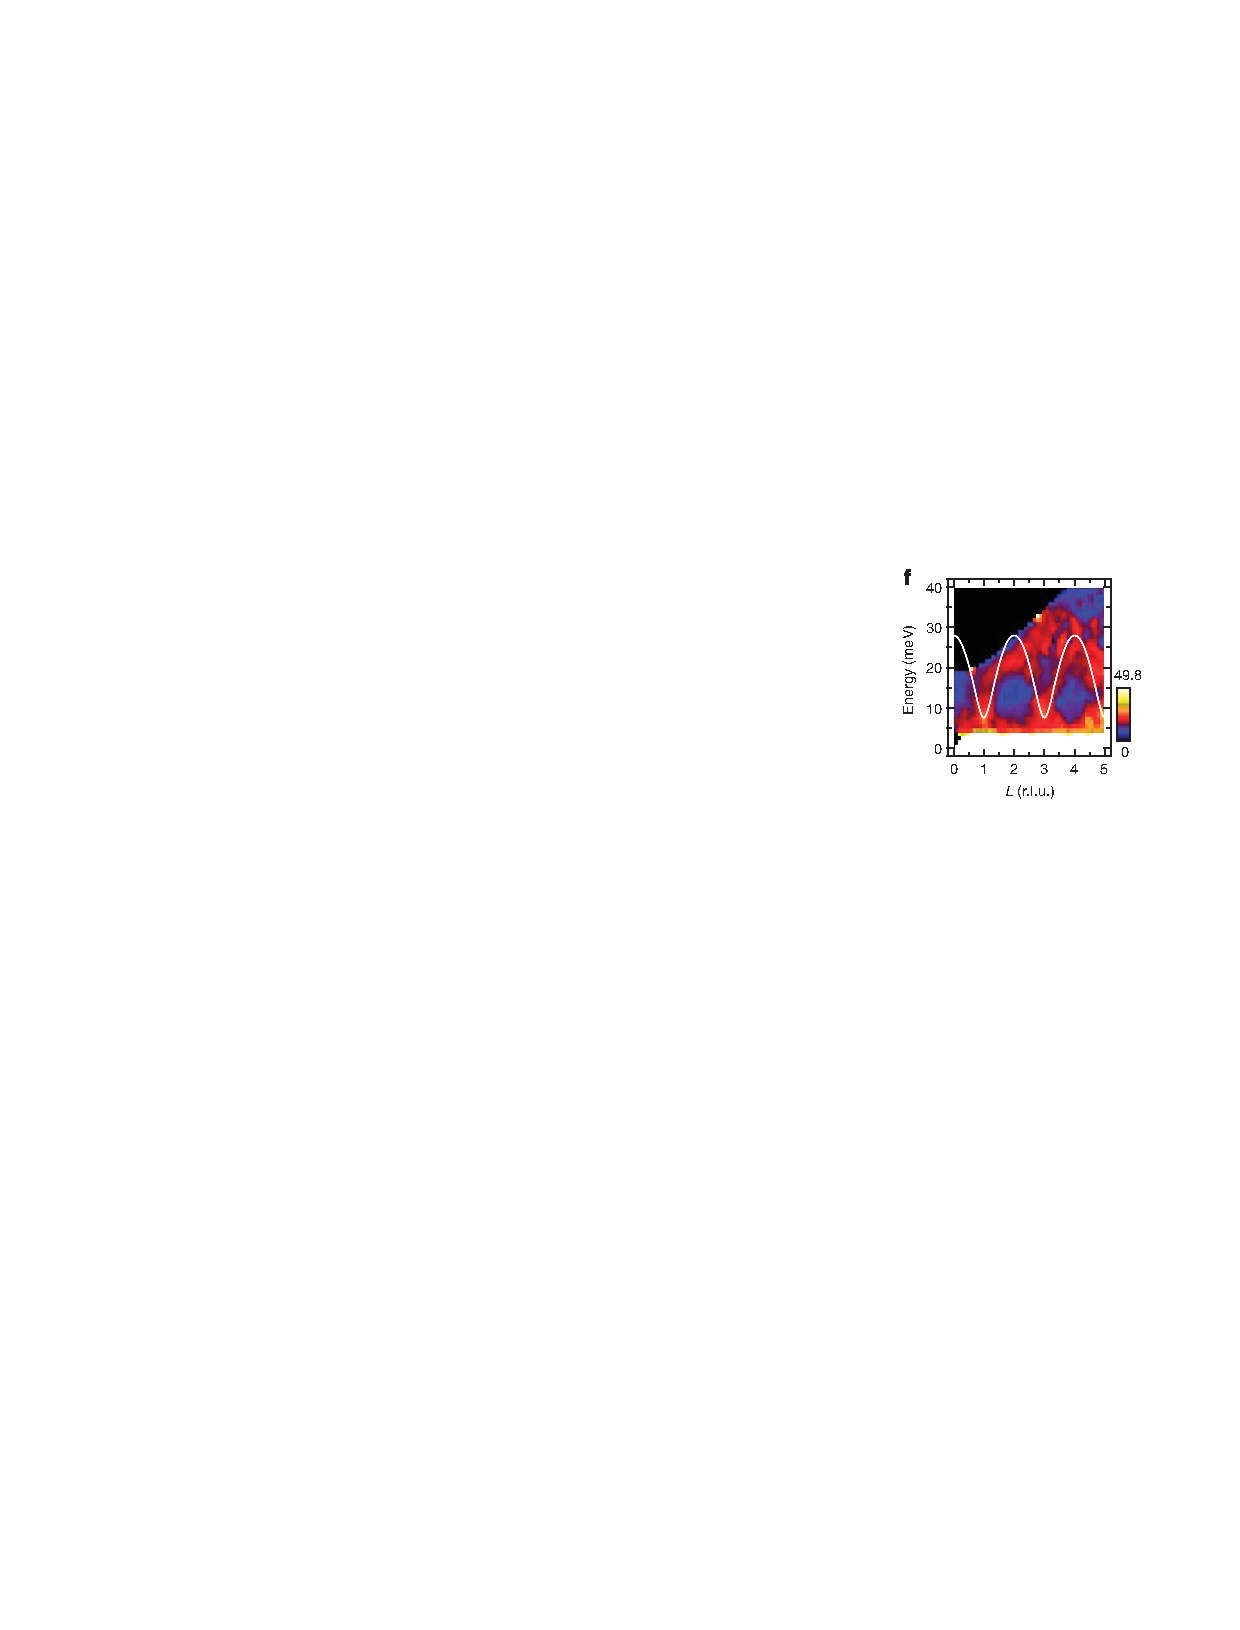
\includegraphics[height=3cm]{../spinexp/spinwaveins}~~~
  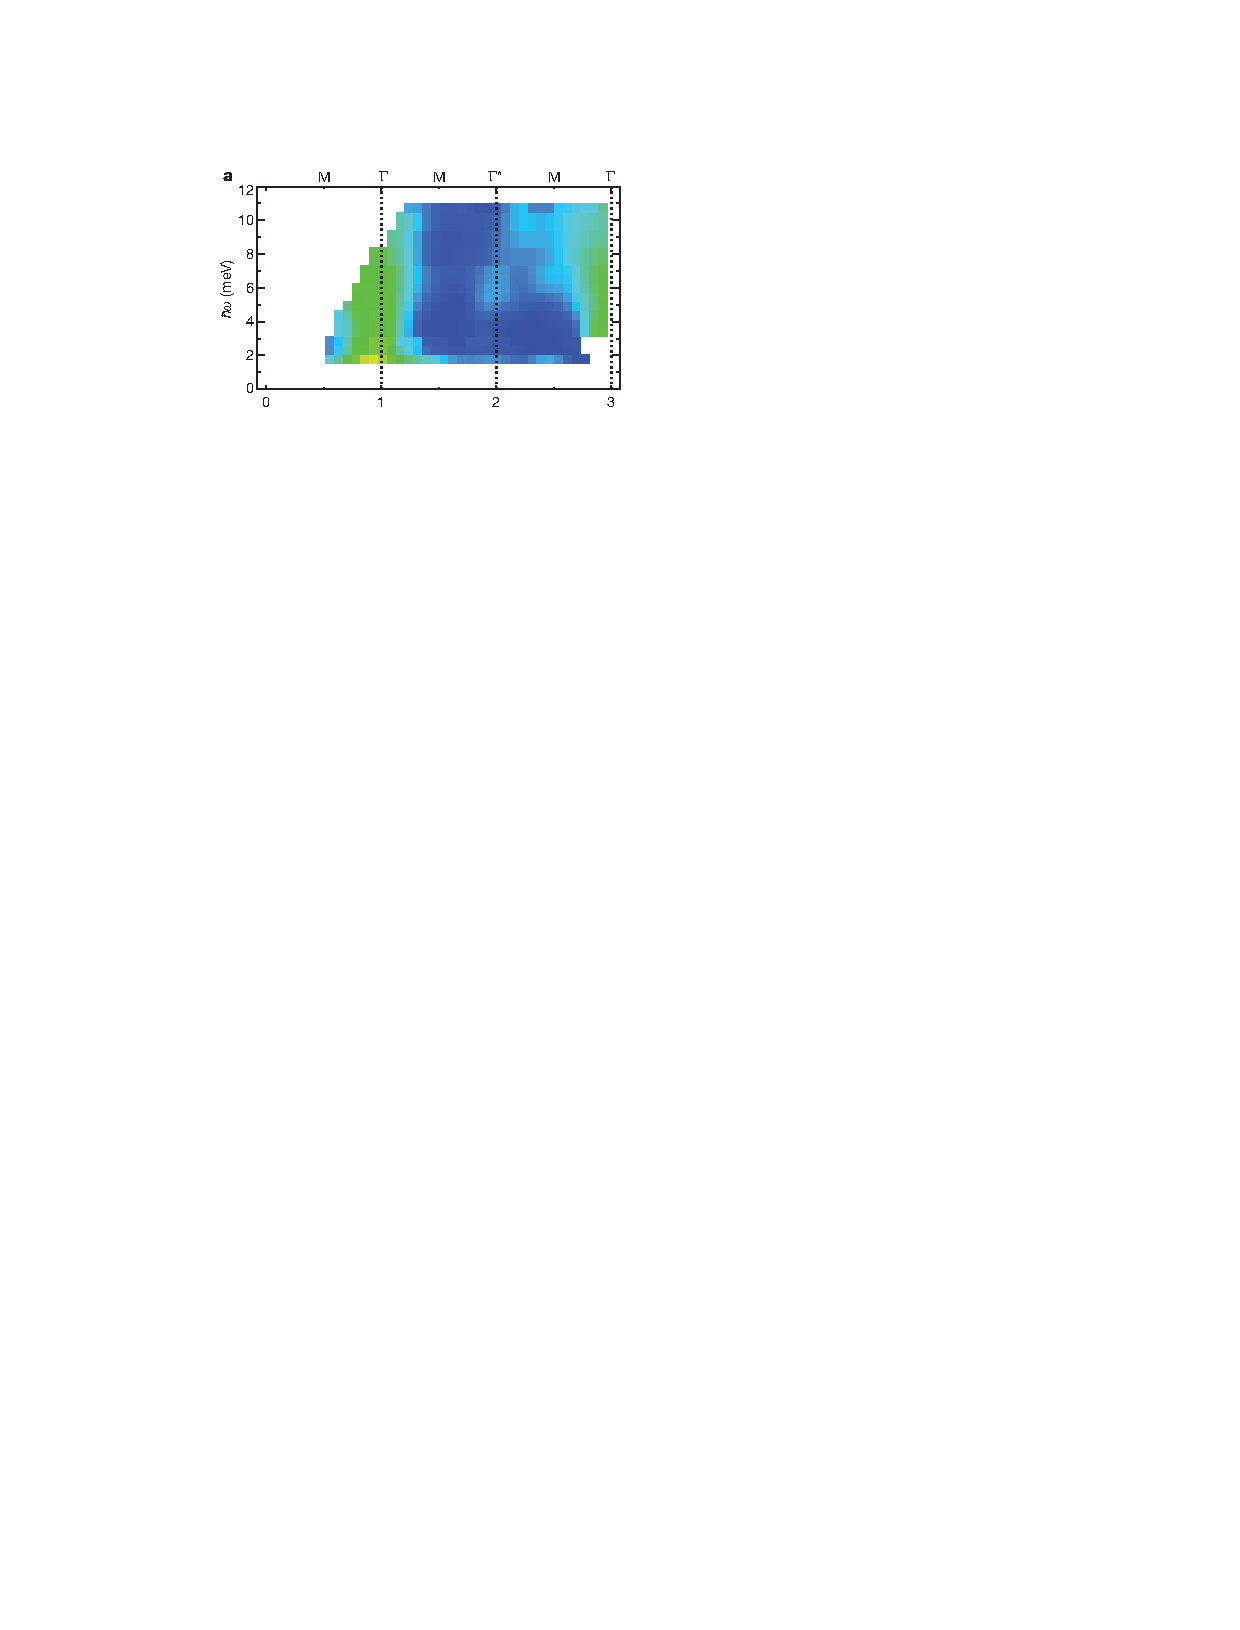
\includegraphics[height=3cm]{../spinexp/continuumins}
\end{center}
\end{frame}

\begin{frame}
\frametitle{Phases and ground state degeneracy}
Possible phases in a quantum spin system:
\begin{enumerate}
  \item<1-4> Trivial paramagnet: no GSD.
  \item<2-> Symmetry-breaking phases: FM, AFM, VBS, etc. GSD due to symmetry breaking.
  \item<3-> Gapped spin liquid: GSD on a torus, due to topological order.
  \item<4-> Gapless spin liquid: GSD due to gapless excitations / topological order.
\end{enumerate}
\action<5>{No-go theorem rules out case 1.}
\end{frame}

\section{Projective representation: symmetry-protected nontrivialness.}

\begin{frame}
\frametitle{Spin-$\frac12$: a quantum object}
\begin{itemize}
  \item Integer spins: 360-degree rotation = +1.
  \item Spin-$\frac12$ object: 360-degree rotation = $-1$.
  \item Spin rotation symmetry is SO(3): all local excitations carry integer spins.
\item SO(3) symmetry $\rightarrow$ $\mathbb D_2=\mathbb Z_2\times\mathbb Z_2$, generated by $X=e^{i\pi S_x}$ and $Z=e^{i\pi S_z}$.
\item SO(3) group algebra: $XZ = ZX$.
\item Spin-$1/2$: $X=i\sigma_x$, $Z=i\sigma_z$. $XZ=-ZX$. Projective representation.
\item Spin-$1/2$: symmetry-protected two-fold degeneracy: $\uparrow$/$\downarrow$.
\end{itemize}
\begin{center}
  \begin{animateinline}{25}
    \multiframe{91}{Ra=45+4}{
    \begin{tikzpicture}[scale=2]
      \draw [white] (-.5, -.5)--(.5, .5);
      \filldraw (0, 0) circle (1pt) node [above] {a};
      \draw [->] (\Ra:-0.2)--(\Ra:0.2);
      \draw [thick, ->] (45: .3) arc (45:\Ra: .3);
    \end{tikzpicture}}
  \end{animateinline}
\end{center}
\end{frame}

\begin{frame}
\frametitle{Projective representation}
\begin{itemize}
  \item A representation: $\phi: G\rightarrow GL(V)$.
  \item Linear representation: all local excitations carry linear representations of $G$.
  \[\phi(g)\phi(h) = \phi(gh).\]
  \item Projective representation: quantum states are defined up to a U(1) phase.
  \[\phi(g)\phi(h)=\omega(g, h)\phi(gh).\]
  \item Group cohomology: $\omega\in H^2[G, \text U(1)]$.
  \item $H^2[G, \text U(1)]$ can be computed by GAP (\url{http://www.gap-system.org}).
  \item All states in the Hilbert space must belong to the same class: either all linear or all projective.
  \item When the Hilbert space transforms projectively, it has symmetry-protected degeneracy.
\end{itemize}
\end{frame}

\begin{frame}
\frametitle{Lieb-Schultz-Mattis-Oshikawa-Hastings Theorem}
\begin{itemize}
\item Symmetry: translation + onsite symmetry. $\mathbb Z^2\times G$, $G = SO(3) \text{ or } \mathbb Z_2^T$.
\item Dimensional reduction: 2D $\rightarrow$ 0D.
\item A projective rep (an odd \# of spin-$\frac12$) per unit cell.
\item On a torus with an odd \# of unit cells: the whole Hilbert space transforms projectively.
\item Must be degenerate, unless symmetry is broken.
\end{itemize}
\begin{center}
  \includegraphics<1>{../dimer/dimer_spin}
\end{center}
\end{frame}

\begin{frame}
\frametitle{Application of LSM Theorem}
\begin{columns}
  \column{.5\textwidth}
\begin{itemize}
\item Haldane conjecture: a half-integer spin chain is gapless.
\item 2D spin-$\frac12$ model.
\begin{itemize}
  \item Square lattice, triangular lattice, kagome lattice.
  \item N\'eel state, valence bond solid state, or quantum spin liquid.
  \item $\kappa$-ET, dmit, herbertsmithite, YbMgGaO, $\cdots$.
  \item Must have an odd \# of spin-$\frac12$ per unit cell.\\
  Counterexample: honeycomb lattice.
\end{itemize}\end{itemize}
\column{.5\textwidth}
\begin{center}
  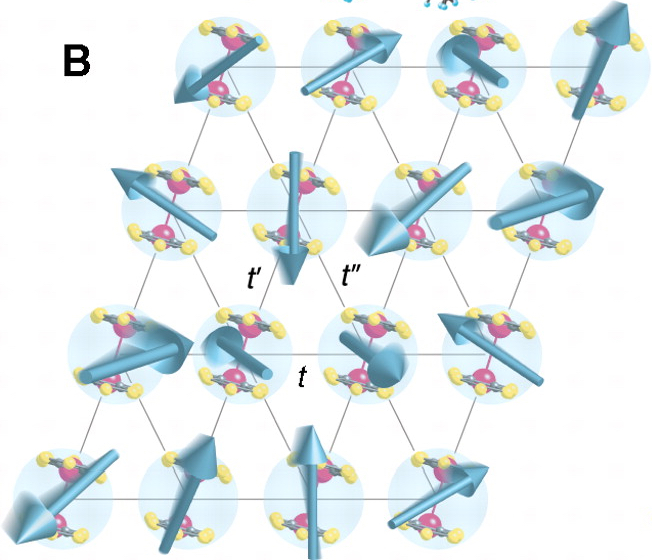
\includegraphics[width=3cm]{../spinexp/dmit}~~~~
  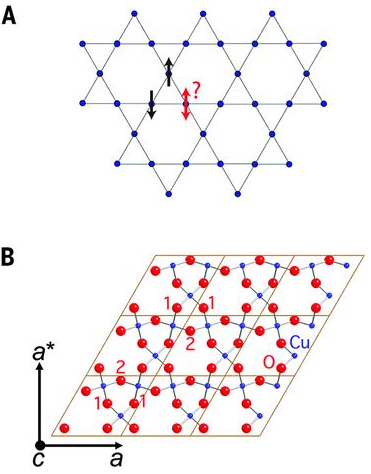
\includegraphics[width=3cm]{../spinexp/herbertsmithite}
\end{center}
\emph{M Yamashita et al, Science \textbf{328} 1246 (2010); \small M Fu et al, Science \textbf{350}, 655 (2015).}
\end{columns}
\end{frame}

\section{Our theorem: using only the space-group symmetry.}

\begin{frame}
\frametitle{Point-group symmetry}
\begin{columns}
\column{.3\textwidth}
\begin{tikzpicture}
\draw [double] (-2, 0)--(2, 0);
\draw [double] (0, -2)--(0, 2);
\node at (0, 0) [diamond, aspect=0.5, fill=mbg, draw] {};
\node at (1, 1) {F};
\node at (-1, 1) [xscale=-1] {F};
\node at (1, -1) [yscale=-1] {F};
\node at (-1, -1) [xscale=-1, yscale=-1] {F};
\end{tikzpicture}
\column{.7\textwidth}
\begin{itemize}
\item Another way of dimensional reduction:\\ point-group symmetry.
\item Example: $G=\mathbb D_2$.
\item Projective representation: $H^2[\mathbb D_2, \text U(1)]=\mathbb Z_2$.
\item Placing a spin-$\frac12$ at rotation center: it carries a projective representation. $M_xM_y=-M_yM_x$.
\item Spins off the center always form linear representations.
\item The whole Hilbert space transforms projectively.
\item Ground state degeneracy protected by $\mathbb D_2$ symmetry.
\end{itemize}
\end{columns}
\end{frame}

\begin{frame}
\frametitle{Example: rectangular lattice}
\begin{itemize}
\item Rectangular lattice: wallpaper group p2mm.
\item Four sets of inequivalent centers. Point group = $\mathbb D_2$.
\item A $\mathbb Z_2$ topological invariant for each rotation center:\\
  $\nu=\pm1$: linear / projective representation.
\item Four $\mathbb Z_2$ topological invariants.
\item $\nu=-1$: symmetry-protected ground state degeneracy.
\end{itemize}
\begin{center}
\includegraphics{../wallpaper/p2mm_enrich}
\end{center}
\end{frame}

\begin{frame}{Other lattices}
  \begin{itemize}
    \item $D_{2,4,6}$ has nontrivial projective reps:
    \[H^2[D_{2,4,6}, \text U(1)] = Z_2.\]
    \item Other point groups does not have projective reps:
    \[H^2[D_3, \text U(1)] = H^2[C_n, \text U(1)] = Z_1.\]
  \end{itemize}
  \begin{table}
    \centering
    \renewcommand{\arraystretch}{1.5}
    \rowcolors{2}{black!20}{}
    \begin{tabularx}{\columnwidth}{xxxxx}
      \rowcolor{mbg}\textcolor{white}{p2mm}
      &\textcolor{white}{c2mm}
      &\textcolor{white}{p4gm}
      &\textcolor{white}{p4mm}
      &\textcolor{white}{p6mm}\\
      \includegraphics[scale=.8]{../wallpaper/p2mm} &
      \includegraphics[scale=.8]{../wallpaper/c2mm} &
      \includegraphics[scale=.8]{../wallpaper/p4gm} &
      \includegraphics[scale=.8]{../wallpaper/p4mm} &
      \includegraphics[scale=.8]{../wallpaper/p6mm}\\
      $4\times$ & $2\times$ & $1\times$ & $3\times$ & $2\times$
    \end{tabularx}
  \end{table}
\end{frame}

\begin{frame}
  \frametitle{Application: checkerboard lattice}
  \begin{columns}
    \column{.3\textwidth}
    \begin{center}
      \includegraphics{../wallpaper/checkerboard}\\
    \end{center}
    \begin{center}
      \includegraphics{../wallpaper/p4mm}
    \end{center}
    \column{.7\textwidth}
    \begin{itemize}
    \item Different interactions on light/dark plaquettes.
    \item Two spin-$\frac12$s per unit cell:\\the original LSM Thm is silent.
    \item Ground state degeneracy protected by the p4mm symmetry.
    \item $J_1$-$J_2$ model on the checkerboard lattices:\\
    models the ``planar-pyrochlore'' materials.
    \end{itemize}
  \end{columns}
\end{frame}

\section{An alternative understanding: a three-dimensional view.}

\begin{frame}
  \frametitle{Symmetry Protected Topological (SPT) states}
  A short introduction: think about Topological Insulator (TI) as an example.
  \begin{itemize}
    \item Bulk is gapped.
    \item No long-range entanglements, no anyons, no ground state degeneracy in the bulk.
    \item Only nontrivial because of symmetries.
    \item Surface has symmetry-protected degeneracy:
    \begin{enumerate}
      \item Surface can be gapped by breaking symmetries.
      \item Surface can be gapless.
      \item Surface can form a gapped topological order, which still has ground-state degeneracy.
    \end{enumerate}
  \end{itemize}
  The conclusion of the no-go theorems looks the same.
\end{frame}

\begin{frame}
  \frametitle{Example: LSM Theorem}
  \begin{itemize}
  \item Physical system: odd \# of spin-$\frac12$ (half-integer spin) per unit cell.
  %\item M Cheng et al, to appear.
  \item ``Anomaly'': Impossible for a 2D spin-1 system.
  \item<2-> Spin-$\frac12$: edge of a spin-1 AKLT chain (1d SPT).
  \item<3-> 2D Stacking of 1D SPT state (AKLT chains).
  \item<3-> Weak 3D SPT: protected by
    $\text{SO}(3)\times T_x\times T_y$.
  \end{itemize}
  \begin{center}
      \includegraphics<1>{../dimer/weak3d_2d_blue}
      \only<2>{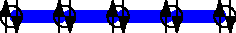
\includegraphics{../dimer/weak3d_aklt_blue}\\=\\\includegraphics{../dimer/weak3d_aklt2_blue}}
      \includegraphics<3>{../dimer/weak3d_3d_blue}
  \end{center}
\end{frame}

\begin{frame}
  \frametitle{Crystal symmetry}
  \begin{itemize}
  \item Bulk:
  \begin{itemize}
    \item Haldane chains located at rotation centers.
    \item 3D topological crystalline insulator (TCI), protected by the wallpaper group.
  \end{itemize}
  \item Surface:
  \begin{itemize}
    \item Spin-$\frac12$s located at rotation centers.
    \item Ground state degeneracy, protected by the wallpaper group.
  \end{itemize}
  \end{itemize}
  \begin{center}
      \includegraphics{../dimer/weak3d_3d_blue}
  \end{center}
\end{frame}

\section{Implication on symmetry fractionalization}

\begin{frame}
  \frametitle{Symmetry fractionalization}
  \begin{block}{Fractional quantum number}
    Magnon carries spin-1 but spinon carries spin-$\frac12$:
       $(e^{i\pi S^z})^2=-1$.
  \end{block}

  \begin{block}{How is this possible?}
    $1$ must carry $XY=ZW$, $a$ can carry $XY=\pm ZW$.\\
    $1=a\times a$, so the extra minus sign cancels out.\\
    Anyons can also carry projective representations of the symmetry group.
  \end{block}
  \begin{center}
    \includegraphics<1>{../dimer/dimer0}
    \includegraphics<2>{../dimer/dimer1}
    \includegraphics<3>{../dimer/dimer5}
  \end{center}
\end{frame}

\begin{frame}
  \frametitle{Anomalous surface topological order}
  \begin{itemize}
    \item Surface of 3D SPT state:
    \begin{enumerate}
      \item Surface can be gapped by breaking symmetries.
      \item Surface can be gapless.
      \item Surface can form a gapped topological order, which still has ground-state degeneracy.
    \end{enumerate}
    \item Example: 3D Topological crystalline insulator, $n=4$.
    \begin{enumerate}
      \item Without interaction: $4\times$Dirac cones.
      \item With interaction: can realized a $\mathbb Z_2$ topological order
      \item Both $e$ and $m$ carries $M^2=-1$.
      \\\emph{\small Y Qi and Liang Fu, PRL 2015.}
    \end{enumerate}
  \end{itemize}
  \begin{center}
    \includegraphics[height=3cm]{../resources/tci}
  \end{center}
\end{frame}

\begin{frame}
  \frametitle{Constraints on symmetry fractionalization}
  \centering \includegraphics[scale=.8]{../dimer/weak3d_3d_blue}~~~~~~~~~\includegraphics[scale=.8]{../dimer/weak3d_2d_blue}
  \begin{itemize}
    \item UV limit: ``SPT surface state''.\\
    spin-$\frac12$ per unit cell.
    \item IR limit: ``anomalous topological order''.\\
    one $e$ particle carrying spin-$\frac12$ per unit cell.
  \end{itemize}
\end{frame}

\begin{frame}
  \frametitle{Spinon's symmetry fractionalization}
  \centering \includegraphics[scale=.8]{../dimer/weak3d_3d_blue}~~~~~~~~~\includegraphics[scale=.8]{../dimer/triangular_lattice}
  \begin{table}
    \centering
    \renewcommand{\arraystretch}{1.5}
    \rowcolors{2}{black!20}{}
    \begin{tabularx}{.8\columnwidth}{xxx}
      \rowcolor{mbg}\textcolor{white}{Label}
      &\textcolor{white}{Relation}
      & \textcolor{white}{$[\omega]^{\text{phys}}=[\omega]^e$}\\
      %Spin & & $\frac12$\\
      $\omega_T$ & $T^2=\pm1$ & $-1$\\
      $\omega_\mu\omega_\sigma/\omega_I$
      & $\sigma\mu=\pm\mu\sigma$ & $+1$ \\
      $\omega_{\mu T}$ & $(\mu T)^2=\pm1$ & $-1$ \\
      $\omega_{\sigma T}$ & $(\sigma T)^2=\pm1$ & $-1$
    \end{tabularx}
  \end{table}
\end{frame}

\section{Conclusion}

\begin{frame}
  \frametitle{Conclusion}
  \begin{columns}
    \column{.3\textwidth}
    \begin{center}
      \includegraphics[scale=1.5]{../wallpaper/p4mm}
    \end{center}
    \column{.7\textwidth}
    \begin{itemize}
      \item Ground state degeneracy protected by point-group symmetries $\mathbb D_{2,4,6}$.
      \item Spin-$\frac12$ at rotation center: must be degenerate.
      \item Can be applied to even \# of spin-$\frac12$ per unit cell.
      \item Can be applied to systems with spin-orbit coupling.
      \item Does not require time-reversal symmetry.
    \end{itemize}
  \end{columns}
\end{frame}

\begin{frame}
  \frametitle{Classification of GAPPED $\mathbb Z_2$ spin liquids}
  Assuming: full SO(3) symmetry + odd # of spin-$\frac12$ per u. c.
  \begin{itemize}
  \item In total: 8 possible states.
  \item YQ, M. Cheng and C. Fang, arXiv:1509.02927; YQ, MC, arXiv:1606.04544.
  \item Only three independent $\mathbb Z_2$ variables, $2^3=8$
    states.
  \item Schwinger-boson (F Wang and A Vishwanath), Schwinger-fermion
    (Y-M Lu, Y Ran and P A Lee) and PEPS (S Jiang and Y Ran).
  \end{itemize}
\end{frame}
\end{document}
